\section{Application}

We propose to apply the model to the specific example of HD209458b detected via transit in 1999 by Charbonneau et al. \parencite{charbonneau_detection_2000}. HD209458b is a Jupiter like planet with a 0.69 Jupiter mass, with a semi-major axis of 0.04747 AU. It is hence a highly irradiated planet, with an effective temperature of around 1400K. This temperature is currently at the limit of the results previously shown in terms of irradiation temperatures but can still be simulated. We wish to estimate it's internal temperature from it's already estimated Radius of 1.38 Jupiter radii. 

\begin{figure}
    \centering
    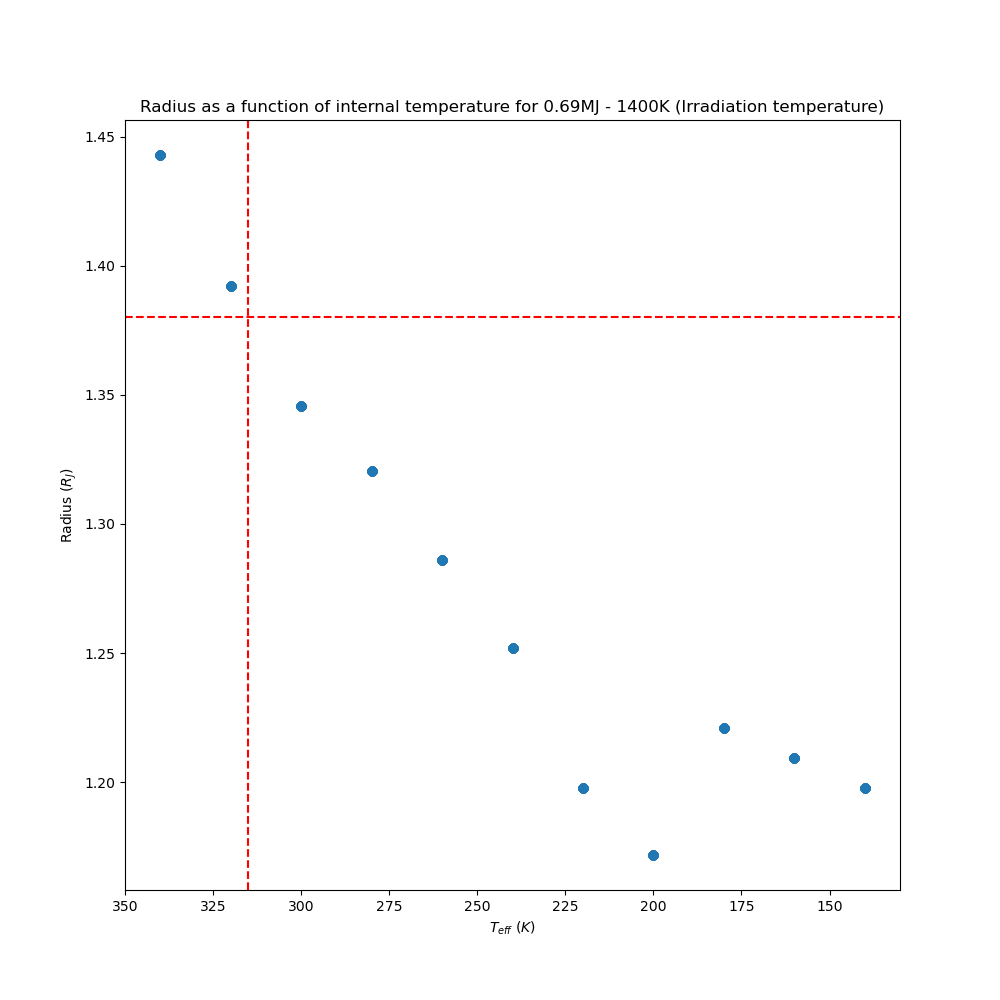
\includegraphics[width=0.48\textwidth]{Images/1400_0.69.png}
    \caption{HD209458b potential evolution curve}
    \label{fig:HD209458b}
\end{figure}

\Cref{fig:HD209458b} indicates that the current internal temperature of HD209458b with the observational parameters is around 320K. We see on this curve that some points appear incorrect, further work is required to understand why some domains of the data are wrong despite the small erreur imposed. However the trend of the whole dataset for the given parameters appears valid. (See annex on interpolation methods)